\section{Hyperbolic Functions}\label{sec:hyperbolic}

The \textbf{hyperbolic functions} are functions that have many applications to mathematics, physics, and engineering. Among many other applications, they are used to describe the formation of satellite rings around planets, to describe the shape of a rope hanging from two points, and have application to the theory of special relativity. This section defines the hyperbolic functions and describes many of their properties, especially their usefulness to calculus.

\mtable{Using trigonometric functions to define points on a circle and hyperbolic functions to define points on a hyperbola.}{fig:hfcircle}{\begin{tikzpicture}
 \begin{axis}[height=\marginparwidth,width=\marginparwidth,
   tick label style={font=\scriptsize},
   axis y line=middle,axis x line=middle,name=myplot,axis on top,
   xtick={-1,1},ytick={-1,1},ymin=-1.1,ymax=1.1,xmin=-1.1,xmax=1.1]
  \addplot [draw={\coloronefill},fill={\coloronefill},domain=0:45] ({cos(x)},{sin(x)})
   -- (axis cs:0,0)--cycle;
  \addplot [draw={\colorone},domain=0:360,thick,smooth,samples=40] ({cos(x)},{sin(x)});
  \filldraw (axis cs:.707,.707) circle (1pt) node [left]%[shift={(4pt,11pt)}]
   {\scriptsize ($\cos \theta$,$\sin \theta$)};
  \draw (axis cs:.6,.25) node {\scriptsize $A=\dfrac{\theta}{2}$};
  \draw (axis cs:-.5,.2) node {\scriptsize $x^2+y^2=1$};
 \end{axis}
% \draw[draw={\colorone}](0,0)circle(1);
 \node [right] at (myplot.right of origin) {\scriptsize $x$};
 \node [above] at (myplot.above origin) {\scriptsize $y$};
\end{tikzpicture}
\vspace{10pt}
\begin{tikzpicture}
 \begin{axis}[height=\marginparwidth,width=\marginparwidth,
   tick label style={font=\scriptsize},
   axis y line=middle,axis x line=middle,name=myplot,axis on top,
   ymin=-3.1,ymax=3.1,xmin=-3.1,xmax=3.1]
  \addplot [draw={\coloronefill},fill={\coloronefill},domain=0:1.6] ({cosh(x)},{sinh(x)})
   -- (axis cs:0,0)--cycle;
  \addplot [draw={\colorone},domain=-2:2,thick,smooth] ({cosh(x)},{sinh(x)});
  \addplot [draw={\colorone},domain=-2:2,thick,smooth] ({-cosh(x)},{sinh(x)});
  \filldraw (axis cs:2.577,2.376) circle (1pt) node [left]
   {\scriptsize ($\cosh \theta$,$\sinh \theta$)};
  \draw (axis cs:2,.6) node {\scriptsize $A=\dfrac{\theta}{2}$};
  \draw (axis cs:-1.75,2.75) node {\scriptsize $x^2-y^2=1$};
 \end{axis}
 \node [right] at (myplot.right of origin) {\scriptsize $x$};
 \node [above] at (myplot.above origin) {\scriptsize $y$};
\end{tikzpicture}}

These functions are sometimes referred to as the ``hyperbolic trigonometric functions'' as there are many connections between them and the standard trigonometric functions. \autoref{fig:hfcircle} demonstrates one such connection. Just as cosine and sine are used to define points on the circle defined by $x^2+y^2=1$, the functions \textbf{hyperbolic cosine} and \textbf{hyperbolic sine} are used to define points on the hyperbola $x^2-y^2=1$.

We begin with their definitions.

\begin{definition}[Hyperbolic Functions]\label{def:hyperbolic_functions}
\mbox{}\\[-2\baselineskip]\parbox[t]{\linewidth}{%
\begin{multicols}{2}\index{hyperbolic function!definition}%
\begin{enumerate}\lxAddClass{columns2}
\item		$\ds \cosh x = \frac{e^x+e^{-x}}2$
\item		$\ds \sinh x = \frac{e^x-e^{-x}}2$
\item		$\ds \tanh x = \frac{\sinh x}{\cosh x}$
\item		$\ds \sech x = \frac{1}{\cosh x}$
\item		$\ds \csch x = \frac{1}{\sinh x}$
\item		$\ds \coth x = \frac{\cosh x}{\sinh x}$
\end{enumerate}
\end{multicols}}
\end{definition}

The hyperbolic functions are graphed in \autoref{fig:hyperbolic}. In the graphs of $\cosh x$ and $\sinh x$, graphs of $e^x/2$ and $e^{-x}/2$ are included with dashed lines. As $x$ gets ``large,'' $\cosh x$ and $\sinh x$ each act like $e^x/2$; when $x$ is a large negative number, $\cosh x$ acts like $e^{-x}/2$ whereas $\sinh x$ acts like $-e^{-x}/2$.

\mnote[1in]{\textbf{Pronunciation Note:} \\
``cosh'' rhymes with ``gosh,'' \\
``sinh'' rhymes with ``pinch,'' and\\
``tanh'' rhymes with ``ranch,'' \\
%``sech'' rhymes with ``fetch,'' and \\
%``coth'' rhymes with ``moth.''
}

Notice the domains of $\tanh x$ and $\sech x$ are $(-\infty,\infty)$, whereas both $\coth x$ and $\csch x$ have vertical asymptotes at $x=0$. Also note the ranges of these functions, especially $\tanh x$: as $x\to\infty$, both $\sinh x$ and $\cosh x$ approach $e^x/2$, hence $\tanh x$ approaches $1$.

\noindent
\begin{minipage}{\linewidth}
\centering
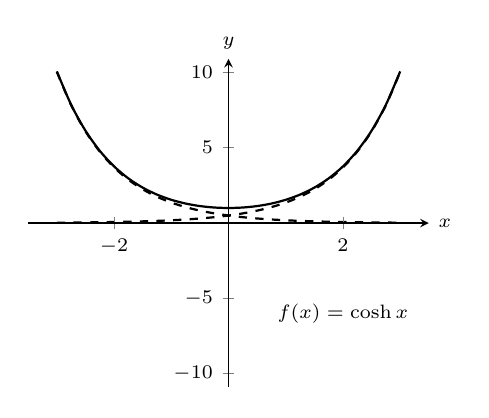
\begin{tikzpicture}
\begin{axis}[width=.55\textwidth,tick label style={font=\scriptsize},
axis y line=middle,axis x line=middle,name=myplot,axis on top,ymin=-10.9,ymax=10.9,
xmin=-3.5,xmax=3.5,scaled ticks=false]
\addplot [draw={\colorone},thick,smooth,domain=-3:3] {cosh(x)};
\draw (axis cs:2,-6) node {\scriptsize $f(x)=\cosh x$};
\addplot [draw={\colortwo},smooth,thick,dashed,domain=-3:3] {exp(x)/2};
\addplot [draw={\colortwo},smooth,thick,dashed,domain=-3:3] {exp(-x)/2};
\end{axis}
\node [right] at (myplot.right of origin) {\scriptsize $x$};
\node [above] at (myplot.above origin) {\scriptsize $y$};
\end{tikzpicture}%
\qquad
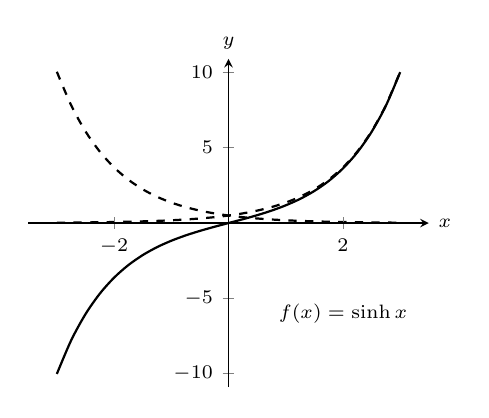
\begin{tikzpicture}
\begin{axis}[width=.55\textwidth,tick label style={font=\scriptsize},
axis y line=middle,axis x line=middle,name=myplot,axis on top,ymin=-10.9,ymax=10.9,
xmin=-3.5,xmax=3.5,scaled ticks=false]
\addplot [draw={\colorone},thick,smooth,domain=-3:3] {sinh(x)};
\draw (axis cs:2,-6) node {\scriptsize $f(x)=\sinh x$};
\addplot [draw={\colortwo},smooth,thick,dashed,domain=-3:3] {exp(x)/2};
\addplot [draw={\colortwo},smooth,thick,dashed,domain=-3:3] {exp(-x)/2};
\end{axis}
\node [right] at (myplot.right of origin) {\scriptsize $x$};
\node [above] at (myplot.above origin) {\scriptsize $y$};
\end{tikzpicture}
\\[20pt]
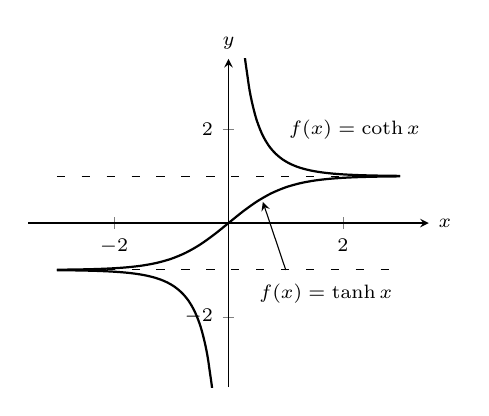
\begin{tikzpicture}
\begin{axis}[width=.55\textwidth,tick label style={font=\scriptsize},
axis y line=middle,axis x line=middle,name=myplot,axis on top,ytick={-2,2},
ymin=-3.5,ymax=3.5,xmin=-3.5,xmax=3.5,scaled ticks=false]
\addplot [draw={\colorone},thick,smooth,domain=-3:3] {tanh(x)};
\draw (axis cs:1.7,-1.5) node {\scriptsize $f(x)=\tanh x$};
\draw (axis cs:2.2,2) node {\scriptsize $f(x)=\coth x$};
\draw [->,>=stealth] (axis cs:1,-1) -- (axis cs:.6,.45);
\addplot [draw={\colortwo},smooth,thick,domain=-3:-.1] {1/tanh(x)};
\addplot [draw={\colortwo},smooth,thick,domain=.1:3] {1/tanh(x)};
\draw [loosely dashed] (axis cs:-3,1) -- (axis cs:3,1);
\draw [loosely dashed] (axis cs:-3,-1) -- (axis cs:3,-1);
\end{axis}
\node [right] at (myplot.right of origin) {\scriptsize $x$};
\node [above] at (myplot.above origin) {\scriptsize $y$};
\end{tikzpicture}%
\qquad
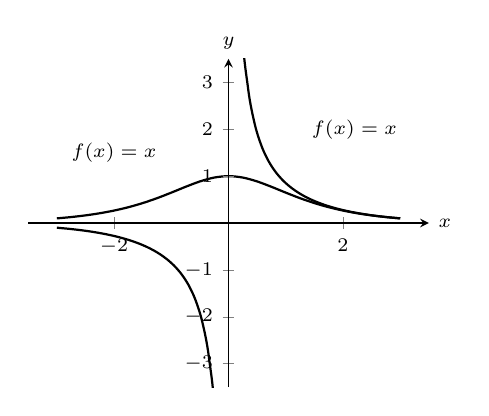
\begin{tikzpicture}
\begin{axis}[width=.55\textwidth,tick label style={font=\scriptsize},
axis y line=middle,axis x line=middle,name=myplot,axis on top,ytick={-3,-2,-1,1,2,3},
ymin=-3.5,ymax=3.5,xmin=-3.5,xmax=3.5,scaled ticks=false]
\addplot [draw={\colorone},thick,smooth,domain=-3:3] {1/cosh(x)};
\draw (axis cs:-2,1.5) node {\scriptsize $f(x)=\sech x$};
\draw (axis cs:2.2,2) node {\scriptsize $f(x)=\csch x$};
\addplot [draw={\colortwo},smooth,thick,domain=-3:-.1] {1/sinh(x)};
\addplot [draw={\colortwo},smooth,thick,domain=.1:3] {1/sinh(x)};
\end{axis}
\node [right] at (myplot.right of origin) {\scriptsize $x$};
\node [above] at (myplot.above origin) {\scriptsize $y$};
\end{tikzpicture}
\captionsetup{type=figure}
\caption{Graphs of the hyperbolic functions.}
\label{fig:hyperbolic}
\end{minipage}

\youtubeVideo{G1C1Z5aTZSQ}{Hyperbolic Functions --- The Basics}

%It is no coincidence that these functions share a name similar to the trigonometric functions. 
The following example explores some of the properties of these functions that bear remarkable resemblance to the properties of their trigonometric counterparts.

\begin{example}[Exploring properties of hyperbolic functions]\label{ex_hf1}
Use \autoref{def:hyperbolic_functions} to rewrite the following expressions.
\begin{multicols}{2}
\begin{enumerate}\lxAddClass{columns2}
\item		$\cosh^2 x-\sinh^2x$
\item		$\tanh^2 x+\sech^2 x$
\item		$2\cosh x\sinh x$
\item		$\frac{\dd}{\dd x}\bigl(\cosh x\bigr)$
\item		$\frac{\dd}{\dd x}\bigl(\sinh x\bigr)$
\item		$\frac{\dd}{\dd x}\bigl(\tanh x\bigr)$
\end{enumerate}
\end{multicols}
\solution
\begin{enumerate}
\item \hfill$\begin{aligned}[t]
 \cosh^2x-\sinh^2x
 &= \left(\frac{e^x+e^{-x}}2\right)^2 -\left(\frac{e^x-e^{-x}}2\right)^2\\
 &= \frac{e^{2x}+2e^xe^{-x} + e^{-2x}}4 - \frac{e^{2x}-2e^xe^{-x} + e^{-2x}}4\\
 &= \frac44=1.
\end{aligned}$\hfill\null\\
So $\cosh^2 x-\sinh^2x=1$.

\item \hfill$\begin{aligned}[t]
 \tanh^2 x+\sech^2 x
 &=\frac{\sinh^2x}{\cosh^2 x} + \frac{1}{\cosh^2 x} \\
 &= \frac{\sinh^2x+1}{\cosh^2 x}\qquad \text{\small Now use identity from \#1.}\\
 &= \frac{\cosh^2 x}{\cosh^2 x} = 1.
\end{aligned}$\hfill\null\\
So $\tanh^2 x+\sech^2 x=1$.

\item \hfill$\begin{aligned}[t]
	2\cosh x\sinh x
	&= 2\left(\frac{e^x+e^{-x}}2\right)\left(\frac{e^x-e^{-x}}2\right) \\
	&= 2 \cdot\frac{e^{2x} - e^{-2x}}4\\
	&= \frac{e^{2x} - e^{-2x}}2 = \sinh (2x).\\
\end{aligned}$\hfill\null\\
Thus $2\cosh x\sinh x = \sinh (2x)$.

\item \hfill$\begin{aligned}[t]
	\frac{\dd}{\dd x}\bigl(\cosh x\bigr)
	&= \frac{\dd}{\dd x}\left(\frac{e^x+e^{-x}}2\right) \\
	&= \frac{e^x-e^{-x}}2\\
	&= \sinh x.
\end{aligned}$\hfill\null\\
So $\frac{\dd}{\dd x}\bigl(\cosh x\bigr) = \sinh x.$
	
\item \hfill$\begin{aligned}[t]
	\frac{\dd}{\dd x}\bigl(\sinh x\bigr)
	&= \frac{\dd}{\dd x}\left(\frac{e^x-e^{-x}}2\right) \\
	&= \frac{e^x+e^{-x}}2\\
	&= \cosh x.
\end{aligned}$\hfill\null\\
So $\frac{\dd}{\dd x}\bigl(\sinh x\bigr) = \cosh x.$

\item \hfill$\begin{aligned}[t]
	\frac{\dd}{\dd x}\bigl(\tanh x\bigr)
	&= \frac{\dd}{\dd x}\left(\frac{\sinh x}{\cosh x}\right) \\
	&= \frac{\cosh x \cosh x - \sinh x \sinh x}{\cosh^2 x}\\
	&= \frac{1}{\cosh^2 x}\\
	&= \sech^2 x.
\end{aligned}$\hfill\null\\
So $\frac{\dd}{\dd x}\bigl(\tanh x\bigr) = \sech^2 x.$
\end{enumerate}
\end{example}

The following Key Idea summarizes many of the important identities relating to hyperbolic functions. Each can be verified by referring back to \autoref{def:hyperbolic_functions}.

{
\tcbset{grow to right by=16em}
\begin{keyidea}[Useful Hyperbolic Function Properties]\label{idea:hyperbolic_identities}
\lxAddClass{columns3}
\begin{minipage}[t]{.33\linewidth}
\textbf{Basic Identities}\par
\index{hyperbolic function!identities}\index{hyperbolic function!derivatives}\index{hyperbolic function!integrals}\index{derivative!hyperbolic funct.}\index{integration!hyperbolic funct.}%
\begin{enumerate}
\item $\cosh^2x-\sinh^2x=1$
\item	$\tanh^2x+\sech^2x=1$
\item	$\coth^2x-\csch^2x = 1$
\item	$\cosh 2x=\cosh^2x+\sinh^2x$
\item	$\sinh 2x = 2\sinh x\cosh x$
\item	$\ds\cosh^2x = \frac{\cosh 2x+1}{2}$
\item $\ds \sinh^2x=\frac{\cosh 2x-1}{2}$
\end{enumerate}
\end{minipage}%
\begin{minipage}[t]{.33\linewidth}
\textbf{Derivatives}
\begin{enumerate}
\item $\frac{\dd}{\dd x}\bigl(\cosh x\bigr) = \sinh x$
\item $\frac{\dd}{\dd x}\bigl(\sinh x\bigr) = \cosh x$
\item $\frac{\dd}{\dd x}\bigl(\tanh x\bigr) = \sech^2 x$
\item $\frac{\dd}{\dd x}\bigl(\sech x\bigr) = -\sech x\tanh x$
\item $\frac{\dd}{\dd x}\bigl(\csch x\bigr) = -\csch x\coth x$
\item $\frac{\dd}{\dd x}\bigl(\coth x\bigr) = -\csch^2x$
\end{enumerate}
\end{minipage}%
\begin{minipage}[t]{.33\linewidth}
\textbf{Integrals}
\begin{enumerate}
\item $\ds\int \cosh x\dd x = \sinh x+C$
\item $\ds\int \sinh x\dd x = \cosh x+C$
\item $\ds\int \tanh x\dd x = \ln(\cosh x) +C$
\item $\ds\int \coth x\dd x = \ln\abs{\sinh x}+C$
\end{enumerate}
\end{minipage}
\end{keyidea}
}

We practice using \autoref{idea:hyperbolic_identities}.

\begin{example}[Derivatives and integrals of hyperbolic functions]\label{ex_hf2}
Evaluate the following derivatives and integrals.\\
\begin{minipage}[t]{.5\linewidth}
\begin{enumerate}
\item		$\ds\frac{\dd}{\dd x}\bigl(\cosh 2x\bigr)$
\item		$\ds\int \sech^2(7t-3)\dd t$
\end{enumerate}
\end{minipage}%
\begin{minipage}[t]{.5\linewidth}
\begin{enumerate}\addtocounter{enumi}{2}
\item		$\ds \int_0^{\ln 2} \cosh x\dd x$
\end{enumerate}
\end{minipage}
\solution
\begin{enumerate}
\item		Using the Chain Rule directly, we have $\frac{\dd}{\dd x} \bigl(\cosh 2x\bigr) = 2\sinh 2x$.

Just to demonstrate that it works, let's also use the Basic Identity found in \autoref{idea:hyperbolic_identities}: $\cosh 2x = \cosh^2x+\sinh^2x$.
\begin{align*}
\frac{\dd}{\dd x}\bigl(\cosh 2x\bigr) = \frac{\dd}{\dd x}\bigl(\cosh^2x+\sinh^2x\bigr)
&= 2\cosh x\sinh x+ 2\sinh x\cosh x\\
&= 4\cosh x\sinh x.
\end{align*}
Using another Basic Identity, we can see that $4\cosh x\sinh x = 2\sinh 2x$. We get the same answer either way.

\item	  We employ substitution, with $u = 7t-3$ and $\dd u = 7\dd t$. Applying
\autoref{idea:hyperbolic_identities} we have:
\[\int \sech^2 (7t-3)\dd t = \frac17\tanh (7t-3) + C.\]

\item \[\int_0^{\ln 2} \cosh x\dd x = \sinh x\Big|_0^{\ln 2} = \sinh (\ln 2) - \sinh 0 = \sinh(\ln 2).\]

We can simplify this last expression as $\sinh x$ is based on exponentials:
\[\sinh(\ln 2) = \frac{e^{\ln 2}-e^{-\ln 2}}2 = \frac{2-1/2}{2} = \frac34.\]
\end{enumerate}
\end{example}

\subsection{Inverse Hyperbolic Functions}

Just as the inverse trigonometric functions are useful in certain integrations, the inverse hyperbolic functions are useful with others. \autoref{fig:hfinverse2} shows the restrictions on the domains to make each function one-to-one and the resulting domains and ranges of their inverse functions. Their graphs are shown in \autoref{fig:hfinverse1}.\index{hyperbolic function!inverse}

Because the hyperbolic functions are defined in terms of exponential functions, their inverses can be expressed in terms of logarithms as shown in \autoref{idea:hyperbolic_log}. It is often more convenient to refer to $\sinh^{-1}x$ than to $\ln\bigl(x+\sqrt{x^2+1}\bigr)$, especially when one is working on theory and does not need to compute actual values. On the other hand, when computations are needed, technology is often helpful but many hand-held calculators lack a \emph{convenient} $\sinh^{-1}x$ button. (Often it can be accessed under a menu system, but not conveniently.) In such a situation, the logarithmic representation is useful. The reader is not encouraged to memorize these, but rather know they exist and know how to use them when needed.

\noindent\begin{minipage}[t]{\linewidth}\noindent%
\captionsetup{type=figure}%
\flushinner{%
\small
\begin{tabular}{ l c c @{\hspace{2em}} c c c }
Function & Domain & Range & Function & Domain & Range \\ \cmidrule(r{2em}){1-3} \cmidrule(l{-1em}){4-6}
$\cosh x$ & $[0,\infty)$ & $[1,\infty)$ &
 $\cosh^{-1} x$ & $[1,\infty)$ & $[0,\infty)$ \\
$\sinh x$ & $(-\infty,\infty)$ & $(-\infty,\infty)$ &
 $\sinh^{-1} x$ & $(-\infty,\infty)$ & $(-\infty,\infty)$\\
$\tanh x$ & $(-\infty,\infty)$ & $(-1,1)$ &
 $\tanh^{-1} x$ & $(-1,1)$ & $(-\infty,\infty)$\\
$\sech x$ & $[0,\infty)$ & $(0,1]$ & $\sech^{-1} x$ & $(0,1]$ & $[0,\infty)$\\
$\csch x$ & $(-\infty,0) \cup (0,\infty)$ & $(-\infty,0) \cup (0,\infty)$ &
 $\csch^{-1} x$ & $(-\infty,0) \cup (0,\infty)$ & $(-\infty,0) \cup (0,\infty)$\\
$\coth x$ & $(-\infty,0) \cup (0,\infty)$ & $(-\infty,-1) \cup (1,\infty)$ &
 $\coth^{-1} x$ & $(-\infty,-1) \cup (1,\infty)$ & $(-\infty,0) \cup (0,\infty)$
\end{tabular}}
\caption{Domains and ranges of the hyperbolic and inverse hyperbolic functions.}
\label{fig:hfinverse2}
\end{minipage}

\noindent\begin{minipage}[t]{\linewidth}\noindent%
\captionsetup{type=figure}%
\flushinner{%
\addtolength{\tabcolsep}{6pt}
\begin{tabular}{cc}
\begin{tikzpicture}
\begin{axis}[width=1.16\marginparwidth,tick label style={font=\scriptsize},
axis y line=middle,axis x line=middle,name=myplot,axis on top,axis equal,
ymin=-.9,ymax=10.9,xmin=-.9,xmax=10.9,scaled ticks=false]
\addplot [draw={\colorone},thick,smooth,domain=0:3] {cosh(x)};
\draw (axis cs:8,4) node {\scriptsize $y=\cosh^{-1} x$};
\draw (axis cs:5.6,10) node {\scriptsize $y=\cosh x$};
\addplot [draw={\colortwo},smooth,thick,domain=0:3] ({cosh(x)},x);
\addplot [dashed,domain=-.5:10] {x};
\end{axis}
\node [right] at (myplot.right of origin) {\scriptsize $x$};
\node [above] at (myplot.above origin) {\scriptsize $y$};
\end{tikzpicture}
&
\begin{tikzpicture}
\begin{axis}[width=1.16\marginparwidth,tick label style={font=\scriptsize},
axis y line=middle,axis x line=middle,name=myplot,axis on top,axis equal,
ymin=-10.9,ymax=10.9,xmin=-10.9,xmax=10.9,scaled ticks=false]
\addplot [draw={\colorone},thick,smooth,domain=-3:3] {sinh(x)};
\draw (axis cs:-6,7) node {\scriptsize $y=\sinh x$};
\draw (axis cs:6,-5) node {\scriptsize $y=\sinh^{-1} x$};
\draw[->,>=stealth] (axis cs:-1,7) -- (axis cs:2,7);
\draw[->,>=stealth] (axis cs:7,-3) -- (axis cs:7,2);
\addplot [draw={\colortwo},smooth,thick,domain=-3:3] ({sinh(x)},x);
\addplot [dashed,domain=-10:10] {x};
\end{axis}
\node [right] at (myplot.right of origin) {\scriptsize $x$};
\node [above] at (myplot.above origin) {\scriptsize $y$};
\end{tikzpicture}
\\[15pt]
\begin{tikzpicture}
\begin{axis}[width=1.16\marginparwidth,tick label style={font=\scriptsize},
axis y line=middle,axis x line=middle,name=myplot,axis on top,xtick={-2,2},
ytick={-2,2},ymin=-3.2,ymax=3.2,xmin=-3.2,xmax=3.2,scaled ticks=false,axis equal]
\addplot [draw={\colortwo},thick,smooth,domain=.348:3] ({1/tanh(x)},x);
\addplot [draw={\colortwo},thick,smooth,domain=-3:-.348] ({1/tanh(x)},x);
\draw (axis cs:2.2,1.5) node {\tiny $y=\coth^{-1} x$};
\draw (axis cs:2.2,-1.5) node {\tiny $y=\tanh^{-1} x$};
\draw [->,>=stealth] (axis cs:1.8,-1.3) -- (axis cs:.2,-.2);
\draw [loosely dashed] (axis cs:-1,-3)--(axis cs:-1,3);
\draw [loosely dashed] (axis cs:1,-3)--(axis cs:1,3);
\addplot [draw={\colorone},smooth,thick,domain=-3.8:3.8] ({tanh(x)},x);
\end{axis}
\node [right] at (myplot.right of origin) {\scriptsize $x$};
\node [above] at (myplot.above origin) {\scriptsize $y$};
\end{tikzpicture}
&
\begin{tikzpicture}
\begin{axis}[width=1.16\marginparwidth,tick label style={font=\scriptsize},
axis y line=middle,axis x line=middle,name=myplot,axis on top,
xtick={-3,-2,-1,1,2,3},ytick={-3,-2,-1,1,2,3},
ymin=-3.5,ymax=3.5,xmin=-3.5,xmax=3.5,scaled ticks=false,axis equal]
\draw (axis cs:1.5,-1.5) node {\tiny $y=\sech^{-1} x$};
\draw (axis cs:-2.2,-1.6) node {\tiny $y=\csch^{-1} x$};
\draw [->,>=latex] (axis cs:1,-1.2) -- (axis cs:1,-.2);
\addplot [draw={\colortwo},smooth,thick,domain=-3:-.3275] ({1/sinh(x)},x);
\addplot [draw={\colortwo},smooth,thick,domain=.3275:3] ({1/sinh(x)},x);
\addplot [draw={\colorone},thick,smooth,domain=0:3] ({1/cosh(x)},x);
\end{axis}
\node [right] at (myplot.right of origin) {\scriptsize $x$};
\node [above] at (myplot.above origin) {\scriptsize $y$};
\end{tikzpicture}
\end{tabular}}
\caption{Graphs of the hyperbolic functions and their inverses.}\label{fig:hfinverse1}
\end{minipage}

Now let's consider the inverses of the hyperbolic functions. We begin with the function $f(x)=\sinh x$. Since $\fp(x)=\cosh x>0$ for all real $x$, $f$ is increasing and must be one-to-one.
% todo Tim once we have an example of finding an inverse in text/07_Inverse_Functions.tex
% We proceed as in \autoref{sec:inv_funcs}:
\begin{align*}\allowdisplaybreaks
y&=\frac{e^x-e^{-x}}2\\
2y&=e^x-e^{-x} \qquad\text{(now multiply by $e^x$)}\\
2ye^x&=e^{2x}-1 \qquad\text{(a quadratic form )}\\
\left(e^x\right)^2-2ye^x-1&=0 \qquad\text{(use the quadratic formula)}\\
e^x&=\frac{2y\pm\sqrt{4y^2+4}}2\\
e^x&=y\pm\sqrt{y^2+1} \qquad\text{(use the fact that $e^x>0$)}\\
e^x&=y+\sqrt{y^2+1}\\
x&=\ln(y+\sqrt{y^2+1})\\
\end{align*}
Finally, interchange the variable to find that
\[\sinh^{-1} x=\ln(x+\sqrt{x^2+1}).\]
In a similar manner we find that the inverses of the other hyperbolic functions are given by:

{
\tcbset{grow to right by=5em} % 5 sufficient
\begin{keyidea}[Logarithmic definitions of Inverse Hyperbolic Functions]\label{idea:hyperbolic_log}
\mbox{}\\[-2\baselineskip]%
\index{hyperbolic function!inverse!logarithmic def.}%
\begin{multicols}{2}
\begin{enumerate}\lxAddClass{columns2}
\item $\ds\cosh^{-1}x=\ln\bigl(x+\sqrt{x^2-1}\bigr)$;\\\null\qquad $x\geq1$
\item $\ds\tanh^{-1}x=\frac12\ln\left(\frac{1+x}{1-x}\right)$;\\\null\qquad$\abs x<1$
\item $\ds\sech^{-1}x=\ln\left(\frac{1+\sqrt{1-x^2}}x\right)$;\\\null\qquad$0<x\leq1$
\item $\ds\sinh^{-1}x=\ln\bigl(x+\sqrt{x^2+1}\bigr)$\\\mbox{}
\item $\ds\coth^{-1}x=\frac12\ln\left(\frac{x+1}{x-1}\right)$;\\\null\qquad$\abs x>1$
\item $\ds\csch^{-1}x=\ln\left(\frac1x+\frac{\sqrt{1+x^2}}{\abs x}\right)$;\\\null\qquad $x\neq0$
\end{enumerate}
\end{multicols}
\end{keyidea}
}

The following Key Ideas give the derivatives and integrals relating to the inverse hyperbolic functions. In \autoref{idea:hyperbolic_inverse_integrals}, both the inverse hyperbolic and logarithmic function representations of the antiderivative are given, based on \autoref{idea:hyperbolic_log}. Again, these latter functions are often more useful than the former.
%Note how inverse hyperbolic functions can be used to solve integrals we used Trigonometric Substitution to solve in \autoref{sec:trig_sub}.



%\mtable{Logarithmic definitions of the inverse hyperbolic functions.}{fig:hfinverse5}{%
%\begin{align*}
%\cosh^{-1}x&=\ln\bigl(x+\sqrt{x^2-1}\bigr);\ x\geq1\\
%\sinh^{-1}x &= \ln\bigl(x+\sqrt{x^2+1}\bigr)\\
%\tanh^{-1}x &= \frac12\ln\left(\frac{1+x}{1-x}\right);\ \abs x<1\\
%\sech^{-1}x &= \ln\left(\frac{1+\sqrt{1-x^2}}x\right);\ 0<x\leq1\\
%\csch^{-1}x &= \ln\left(\frac1x+\frac{\sqrt{1+x^2}}{\abs x}\right);\ x\neq0\\
%\coth^{-1}x &= \frac12\ln\left(\frac{x+1}{x-1}\right);\ \abs x>1
%\end{align*}
%}

{
\tcbset{grow to right by=3em}
\begin{keyidea}[Derivatives Involving Inverse Hyperbolic Functions]\label{idea:hyperbolic_inverse_derivatives}
\index{hyperbolic function!inverse!derivative}\index{derivative!inverse hyper.}
\mbox{}\\[-2\baselineskip]\parbox[t]{\linewidth}{%
\begin{multicols}{2}
\begin{enumerate}\lxAddClass{columns2}
\item $\ds\frac\dd{\dd x}\bigl(\cosh^{-1}x\bigr)=\frac1{\sqrt{x^2-1}}$;\\\null\qquad$x>1$
\item $\ds\frac\dd{\dd x}\bigl(\sinh^{-1}x\bigr)=\frac1{\sqrt{x^2+1}}$\\\vphantom{$x\ne0$}
\item $\ds\frac\dd{\dd x}\bigl(\tanh^{-1}x\bigr)=\frac1{1-x^2}$;\\\null\qquad$\abs x<1$
\item $\ds\frac\dd{\dd x}\bigl(\sech^{-1}x\bigr)=\frac{-1}{x\sqrt{1-x^2}}$;\\\null\qquad$0<x<1$
\item $\ds\frac\dd{\dd x}\bigl(\csch^{-1}x\bigr)=\frac{-1}{\abs x\sqrt{1+x^2}}$;\\\null\qquad$x\neq0$
\item $\ds\frac\dd{\dd x}\bigl(\coth^{-1}x\bigr)=\frac1{1-x^2}$;\\\null\qquad$\abs x>1$
\end{enumerate}
\end{multicols}}
\end{keyidea}}

{
\tcbset{grow to right by=9.5em}
\addtolength{\tabcolsep}{-.2em}
% 9.5em / -.2em sufficient
\begin{keyidea}[Integrals Involving Inverse Hyperbolic Functions]\label{idea:hyperbolic_inverse_integrals}
\index{integration!inverse hyper.}\index{hyperbolic function!inverse!integration}%
\begin{anywhereenum}
\renewcommand{\arraystretch}{2.5}
\begin{tabular}{lll}
\item $\ds\int\frac1{\sqrt{x^2-a^2}}\dd x$ & $\ds{}=\cosh^{-1}\left(\frac xa\right)+C$; $0<a<\abs x$ & $\ds{}=\ln\abs{x+\sqrt{x^2-a^2}}+C$ \\
\item $\ds\int\frac1{\sqrt{x^2+a^2}}\dd x$ & $\ds{}=\sinh^{-1}\left(\frac xa\right)+C$; $a>0$ & $\ds{}=\ln\left(x+\sqrt{x^2+a^2}\right)+C$ \\
\item $\ds\int\frac1{a^2-x^2}\dd x$ & $\ds{}=\begin{cases}
\frac1a\tanh^{-1}\left(\frac xa\right)+C & \abs x<\abs a \\
\frac1a\coth^{-1}\left(\frac xa\right)+C & \abs a<\abs x
\end{cases}$ & $\ds{}=\frac1{2a}\ln\abs{\frac{a+x}{a-x}}+C$ \\
\item $\ds\int\frac1{x\sqrt{a^2-x^2}}\dd x$ & $\ds{}=-\frac1a\sech^{-1}\left(\frac xa\right)+C$; $0<x<a$ & $\ds{}=\frac1a\ln\left(\frac{x}{a+\sqrt{a^2-x^2}}\right)+C$ \\
%\item $\ds\int\frac1{x\sqrt{a^2-x^2}}\dd x$ & $\ds{}=-\frac1a\sech^{-1}\left(\frac xa\right)+C$ & $\ds{}=\frac1a\ln\left(\frac{x}{a+\sqrt{a^2-x^2}}\right)+C$ \\[\defaultaddspace]
%&\null\hfill{$\scriptstyle0<x<a$}\\[\defaultaddspace]
\item $\ds\int\frac1{x\sqrt{x^2+a^2}}\dd x$ & $\ds{}=-\frac1a\csch^{-1}\abs{\frac xa}+C$; $x\neq 0,\ a>0$ & $\ds{}=\frac1a\ln\abs{\frac{x}{a+\sqrt{a^2+x^2}}}+C$\\
%\item $\ds\int\frac1{x\sqrt{x^2+a^2}}\dd x$ & $\ds{}=-\frac1a\csch^{-1}\abs{\frac xa}+C$ & $\ds{}=\frac1a\ln\abs{\frac{x}{a+\sqrt{a^2+x^2}}}+C$\\[\defaultaddspace]
%&\null\hfill{$\scriptstyle x\neq 0,\ a>0$}
\end{tabular}
\end{anywhereenum}
\end{keyidea}}

We practice using the derivative and integral formulas in the following example.

\begin{example}[Derivatives and integrals involving inverse hyperbolic functions]\label{ex_hf3}
Evaluate the following.
\begin{multicols}{2}
\begin{enumerate}\lxAddClass{columns2}
\item	$\ds \frac{\dd}{\dd x}\left[\cosh^{-1}\left(\frac{3x-2}{5}\right)\right]$
\item	$\ds \int\frac{1}{x^2-1}\dd x$
\item	$\ds \int \frac{1}{\sqrt{9x^2+10}}\dd x$
\item[]
\end{enumerate}
\end{multicols}
\solution
\begin{enumerate}
\item	Applying \autoref{idea:hyperbolic_inverse_derivatives} with the Chain Rule gives:
		\[\frac{\dd}{\dd x}\left[\cosh^{-1}\left(\frac{3x-2}5\right)\right] = \frac{1}{\sqrt{\left(\frac{3x-2}5\right)^2-1}}\cdot\frac35.\]

\item		Multiplying the numerator and denominator by $(-1)$ gives 
a %: $\ds \int \frac{1}{x^2-1}\dd x = \int \frac{-1}{1-x^2}\dd x$. The
second integral can be solved with a direct application of item \#3 from \autoref{idea:hyperbolic_inverse_integrals}, with $a=1$. Thus
\begin{align}
\int \frac{1}{x^2-1}\dd x &= -\int \frac{1}{1-x^2}\dd x \notag \\
		&= \begin{cases}-\tanh^{-1}\left(x\right)+C & x^2<1 \\
-\coth^{-1}\left(x\right)+C & 1<x^2 \end{cases} \notag\\
     &=-\frac12\ln\abs{\frac{x+1}{x-1}}+C\notag\\
     &=\frac12\ln\abs{\frac{x-1}{x+1}}+C.\label{eq:hf3}
     \end{align}

%We should note that this exact problem was solved at the beginning of \autoref{sec:partial_fraction}. In that example the answer was given as $\frac12\ln\abs{x-1}-\frac12\ln\abs{x+1}+C.$ Note that this is equivalent to the answer given in \autoeqref{eq:hf3}, as $\ln(a/b) = \ln a - \ln b$.

%The key to linking the two seemingly different answers together is \autoref{fig:hfinverse5}, where the logarithmic definitions of the inverse hyperbolic functions are given. Note that the definitions of $\tanh^{-1}x$ and $\coth^{-1}x$ are very similar; the conditions placed on $\abs x$ ensure that the argument of $\ln$ is always positive. Thus one could say 
%\[\frac12\ln\abs{\frac{x+1}{x-1}} = \begin{cases}\tanh^{-1}x+C & \abs x<1 \\ \\
%\coth^{-1}x+C & \abs x>1 \end{cases}.\]
%
%We reconcile the two answers by returning to \autoeqref{eq:hf3} and continuing:
%\begin{align*}
%\int \frac{1}{x^2-1}\dd x &= \int \frac{-1}{1-x^2}\dd x \\
%			&= \begin{cases}-\frac1a\tanh^{-1}\left(\frac xa\right)+C & x^2<a^2 \\ \\
%-\frac1a\coth^{-1}\left(\frac xa\right)+C & a^2<x^2 \end{cases}\\
%			&= -\frac12\ln\abs{\frac{x+1}{x-1}}+C \\
%			&= -\frac12\ln\abs{x+1} + \frac12\ln\abs{x-1} +C,
%\end{align*}
%matching the answer previously obtained.

\item		This requires a substitution, then item \#2 of \autoref{idea:hyperbolic_inverse_integrals} can be applied.

Let $u = 3x$, hence $\dd u = 3\dd x$. We have 
\begin{align*}
	\int \frac{1}{\sqrt{9x^2+10}}\dd x
	&= \frac13\int\frac{1}{\sqrt{u^2+10}}\dd u.
	\intertext{Note $a^2=10$, hence $a = \sqrt{10}.$ Now apply the integral rule.}
	 &= \frac13 \sinh^{-1}\left(\frac{3x}{\sqrt{10}}\right) + C \\
	 &= \frac13 \ln \abs{3x+\sqrt{9x^2+10}}+C.
\end{align*}
\end{enumerate}
\end{example}

This section covers a lot of ground. New functions were introduced, along with some of their fundamental identities, their derivatives and antiderivatives, their inverses, and the derivatives and antiderivatives of these inverses. Four Key Ideas were presented, each including quite a bit of information.

Do not view this section as containing a source of information to be memorized, but rather as a reference for future problem solving. \autoref{idea:hyperbolic_inverse_integrals} contains perhaps the most useful information. Know the integration forms it helps evaluate and understand how to use the inverse hyperbolic answer and the logarithmic answer.

The next section takes a brief break from demonstrating new integration techniques. It instead demonstrates a technique of evaluating limits that return indeterminate forms. This technique will be useful in \autoref{sec:improper_integration}, where limits will arise in the evaluation of certain definite integrals.


\printexercises{exercises/06-05-exercises}
